% Created by tikzDevice version 0.7.0 on 2014-12-22 11:52:37
% !TEX encoding = UTF-8 Unicode
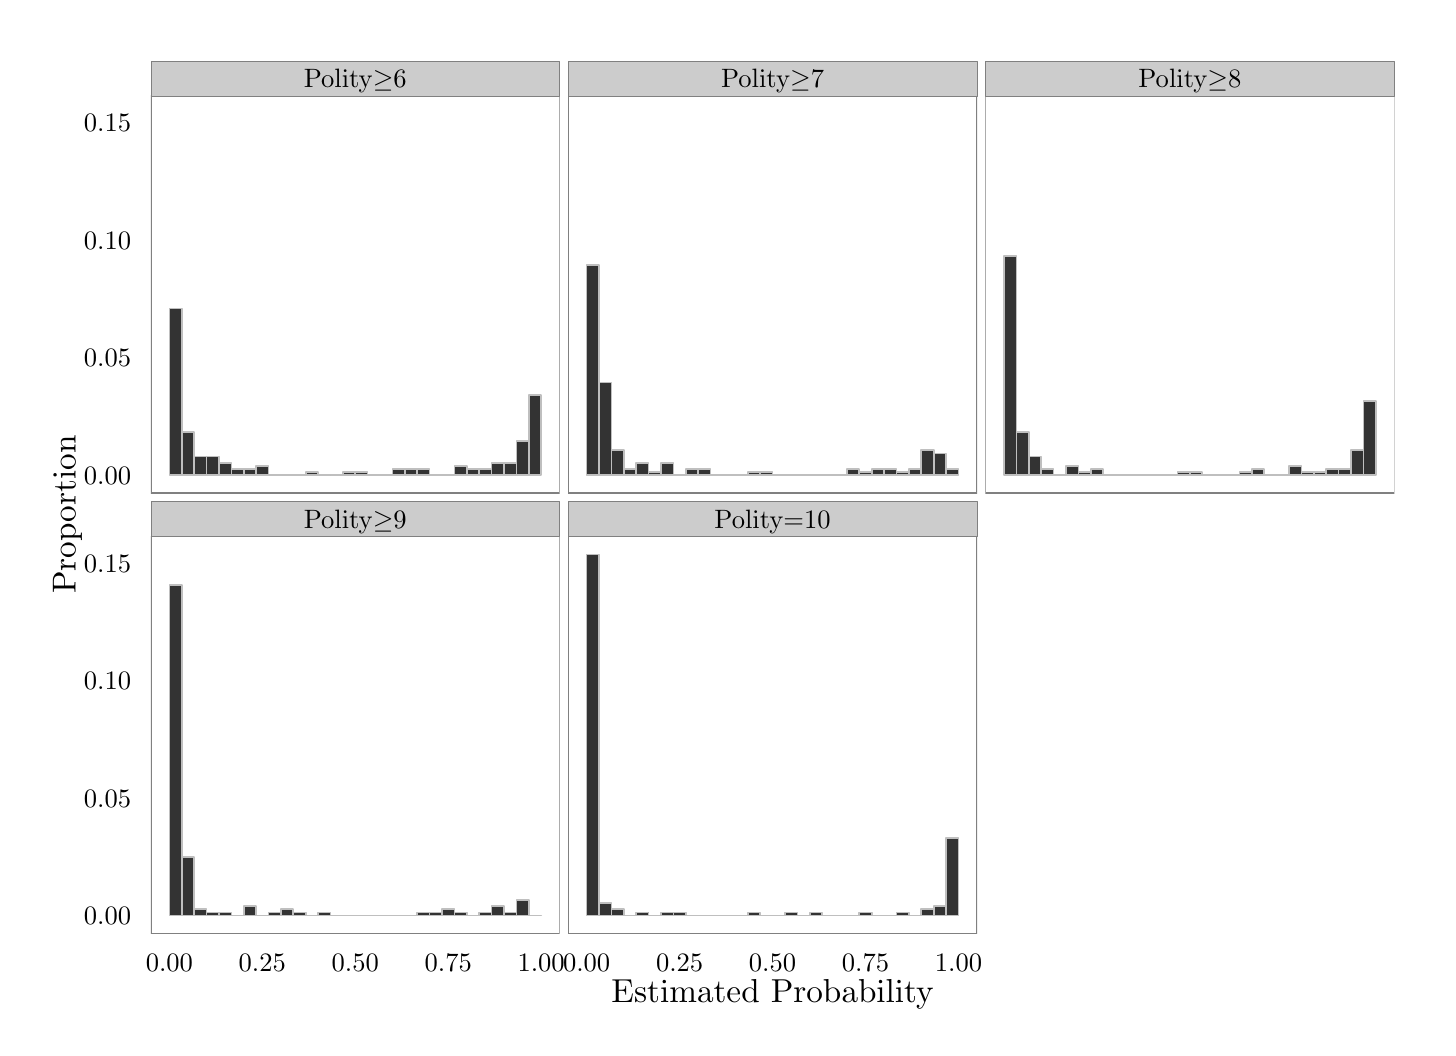
\begin{tikzpicture}[x=1pt,y=1pt]
\definecolor[named]{fillColor}{rgb}{1.00,1.00,1.00}
\path[use as bounding box,fill=fillColor,fill opacity=0.00] (0,0) rectangle (505.89,361.35);
\begin{scope}
\path[clip] (  0.00,  0.00) rectangle (505.89,361.35);
\definecolor[named]{drawColor}{rgb}{1.00,1.00,1.00}
\definecolor[named]{fillColor}{rgb}{1.00,1.00,1.00}

\path[draw=drawColor,line width= 0.6pt,line join=round,line cap=round,fill=fillColor] (  0.00,  0.00) rectangle (505.89,361.35);
\end{scope}
\begin{scope}
\path[clip] ( 44.49,193.18) rectangle (192.26,336.67);
\definecolor[named]{fillColor}{rgb}{1.00,1.00,1.00}

\path[fill=fillColor] ( 44.49,193.18) rectangle (192.26,336.67);
\definecolor[named]{drawColor}{rgb}{0.75,0.75,0.75}
\definecolor[named]{fillColor}{rgb}{0.20,0.20,0.20}

\path[draw=drawColor,line width= 0.6pt,line join=round,fill=fillColor] ( 51.20,199.70) rectangle ( 55.68,259.91);

\path[draw=drawColor,line width= 0.6pt,line join=round,fill=fillColor] ( 55.68,199.70) rectangle ( 60.16,215.31);

\path[draw=drawColor,line width= 0.6pt,line join=round,fill=fillColor] ( 60.16,199.70) rectangle ( 64.64,206.39);

\path[draw=drawColor,line width= 0.6pt,line join=round,fill=fillColor] ( 64.64,199.70) rectangle ( 69.12,206.39);

\path[draw=drawColor,line width= 0.6pt,line join=round,fill=fillColor] ( 69.12,199.70) rectangle ( 73.59,204.16);

\path[draw=drawColor,line width= 0.6pt,line join=round,fill=fillColor] ( 73.59,199.70) rectangle ( 78.07,201.93);

\path[draw=drawColor,line width= 0.6pt,line join=round,fill=fillColor] ( 78.07,199.70) rectangle ( 82.55,201.93);

\path[draw=drawColor,line width= 0.6pt,line join=round,fill=fillColor] ( 82.55,199.70) rectangle ( 87.03,203.04);

\path[draw=drawColor,line width= 0.6pt,line join=round,fill=fillColor] ( 87.03,199.70) rectangle ( 91.51,199.70);

\path[draw=drawColor,line width= 0.6pt,line join=round,fill=fillColor] ( 91.51,199.70) rectangle ( 95.98,199.70);

\path[draw=drawColor,line width= 0.6pt,line join=round,fill=fillColor] ( 95.98,199.70) rectangle (100.46,199.70);

\path[draw=drawColor,line width= 0.6pt,line join=round,fill=fillColor] (100.46,199.70) rectangle (104.94,200.81);

\path[draw=drawColor,line width= 0.6pt,line join=round,fill=fillColor] (104.94,199.70) rectangle (109.42,199.70);

\path[draw=drawColor,line width= 0.6pt,line join=round,fill=fillColor] (109.42,199.70) rectangle (113.90,199.70);

\path[draw=drawColor,line width= 0.6pt,line join=round,fill=fillColor] (113.90,199.70) rectangle (118.37,200.81);

\path[draw=drawColor,line width= 0.6pt,line join=round,fill=fillColor] (118.37,199.70) rectangle (122.85,200.81);

\path[draw=drawColor,line width= 0.6pt,line join=round,fill=fillColor] (122.85,199.70) rectangle (127.33,199.70);

\path[draw=drawColor,line width= 0.6pt,line join=round,fill=fillColor] (127.33,199.70) rectangle (131.81,199.70);

\path[draw=drawColor,line width= 0.6pt,line join=round,fill=fillColor] (131.81,199.70) rectangle (136.29,201.93);

\path[draw=drawColor,line width= 0.6pt,line join=round,fill=fillColor] (136.29,199.70) rectangle (140.77,201.93);

\path[draw=drawColor,line width= 0.6pt,line join=round,fill=fillColor] (140.77,199.70) rectangle (145.24,201.93);

\path[draw=drawColor,line width= 0.6pt,line join=round,fill=fillColor] (145.24,199.70) rectangle (149.72,199.70);

\path[draw=drawColor,line width= 0.6pt,line join=round,fill=fillColor] (149.72,199.70) rectangle (154.20,199.70);

\path[draw=drawColor,line width= 0.6pt,line join=round,fill=fillColor] (154.20,199.70) rectangle (158.68,203.04);

\path[draw=drawColor,line width= 0.6pt,line join=round,fill=fillColor] (158.68,199.70) rectangle (163.16,201.93);

\path[draw=drawColor,line width= 0.6pt,line join=round,fill=fillColor] (163.16,199.70) rectangle (167.63,201.93);

\path[draw=drawColor,line width= 0.6pt,line join=round,fill=fillColor] (167.63,199.70) rectangle (172.11,204.16);

\path[draw=drawColor,line width= 0.6pt,line join=round,fill=fillColor] (172.11,199.70) rectangle (176.59,204.16);

\path[draw=drawColor,line width= 0.6pt,line join=round,fill=fillColor] (176.59,199.70) rectangle (181.07,211.96);

\path[draw=drawColor,line width= 0.6pt,line join=round,fill=fillColor] (181.07,199.70) rectangle (185.55,228.69);
\definecolor[named]{drawColor}{rgb}{0.50,0.50,0.50}

\path[draw=drawColor,line width= 0.6pt,line join=round,line cap=round] ( 44.49,193.18) rectangle (192.26,336.67);
\end{scope}
\begin{scope}
\path[clip] (195.28,193.18) rectangle (343.05,336.67);
\definecolor[named]{fillColor}{rgb}{1.00,1.00,1.00}

\path[fill=fillColor] (195.28,193.18) rectangle (343.05,336.67);
\definecolor[named]{drawColor}{rgb}{0.75,0.75,0.75}
\definecolor[named]{fillColor}{rgb}{0.20,0.20,0.20}

\path[draw=drawColor,line width= 0.6pt,line join=round,fill=fillColor] (201.99,199.70) rectangle (206.47,275.52);

\path[draw=drawColor,line width= 0.6pt,line join=round,fill=fillColor] (206.47,199.70) rectangle (210.95,233.15);

\path[draw=drawColor,line width= 0.6pt,line join=round,fill=fillColor] (210.95,199.70) rectangle (215.43,208.62);

\path[draw=drawColor,line width= 0.6pt,line join=round,fill=fillColor] (215.43,199.70) rectangle (219.91,201.93);

\path[draw=drawColor,line width= 0.6pt,line join=round,fill=fillColor] (219.91,199.70) rectangle (224.38,204.16);

\path[draw=drawColor,line width= 0.6pt,line join=round,fill=fillColor] (224.38,199.70) rectangle (228.86,200.81);

\path[draw=drawColor,line width= 0.6pt,line join=round,fill=fillColor] (228.86,199.70) rectangle (233.34,204.16);

\path[draw=drawColor,line width= 0.6pt,line join=round,fill=fillColor] (233.34,199.70) rectangle (237.82,199.70);

\path[draw=drawColor,line width= 0.6pt,line join=round,fill=fillColor] (237.82,199.70) rectangle (242.30,201.93);

\path[draw=drawColor,line width= 0.6pt,line join=round,fill=fillColor] (242.30,199.70) rectangle (246.77,201.93);

\path[draw=drawColor,line width= 0.6pt,line join=round,fill=fillColor] (246.77,199.70) rectangle (251.25,199.70);

\path[draw=drawColor,line width= 0.6pt,line join=round,fill=fillColor] (251.25,199.70) rectangle (255.73,199.70);

\path[draw=drawColor,line width= 0.6pt,line join=round,fill=fillColor] (255.73,199.70) rectangle (260.21,199.70);

\path[draw=drawColor,line width= 0.6pt,line join=round,fill=fillColor] (260.21,199.70) rectangle (264.69,200.81);

\path[draw=drawColor,line width= 0.6pt,line join=round,fill=fillColor] (264.69,199.70) rectangle (269.17,200.81);

\path[draw=drawColor,line width= 0.6pt,line join=round,fill=fillColor] (269.17,199.70) rectangle (273.64,199.70);

\path[draw=drawColor,line width= 0.6pt,line join=round,fill=fillColor] (273.64,199.70) rectangle (278.12,199.70);

\path[draw=drawColor,line width= 0.6pt,line join=round,fill=fillColor] (278.12,199.70) rectangle (282.60,199.70);

\path[draw=drawColor,line width= 0.6pt,line join=round,fill=fillColor] (282.60,199.70) rectangle (287.08,199.70);

\path[draw=drawColor,line width= 0.6pt,line join=round,fill=fillColor] (287.08,199.70) rectangle (291.56,199.70);

\path[draw=drawColor,line width= 0.6pt,line join=round,fill=fillColor] (291.56,199.70) rectangle (296.03,199.70);

\path[draw=drawColor,line width= 0.6pt,line join=round,fill=fillColor] (296.03,199.70) rectangle (300.51,201.93);

\path[draw=drawColor,line width= 0.6pt,line join=round,fill=fillColor] (300.51,199.70) rectangle (304.99,200.81);

\path[draw=drawColor,line width= 0.6pt,line join=round,fill=fillColor] (304.99,199.70) rectangle (309.47,201.93);

\path[draw=drawColor,line width= 0.6pt,line join=round,fill=fillColor] (309.47,199.70) rectangle (313.95,201.93);

\path[draw=drawColor,line width= 0.6pt,line join=round,fill=fillColor] (313.95,199.70) rectangle (318.42,200.81);

\path[draw=drawColor,line width= 0.6pt,line join=round,fill=fillColor] (318.42,199.70) rectangle (322.90,201.93);

\path[draw=drawColor,line width= 0.6pt,line join=round,fill=fillColor] (322.90,199.70) rectangle (327.38,208.62);

\path[draw=drawColor,line width= 0.6pt,line join=round,fill=fillColor] (327.38,199.70) rectangle (331.86,207.50);

\path[draw=drawColor,line width= 0.6pt,line join=round,fill=fillColor] (331.86,199.70) rectangle (336.34,201.93);
\definecolor[named]{drawColor}{rgb}{0.50,0.50,0.50}

\path[draw=drawColor,line width= 0.6pt,line join=round,line cap=round] (195.28,193.18) rectangle (343.05,336.67);
\end{scope}
\begin{scope}
\path[clip] (346.07,193.18) rectangle (493.85,336.67);
\definecolor[named]{fillColor}{rgb}{1.00,1.00,1.00}

\path[fill=fillColor] (346.07,193.18) rectangle (493.85,336.67);
\definecolor[named]{drawColor}{rgb}{0.75,0.75,0.75}
\definecolor[named]{fillColor}{rgb}{0.20,0.20,0.20}

\path[draw=drawColor,line width= 0.6pt,line join=round,fill=fillColor] (352.78,199.70) rectangle (357.26,278.86);

\path[draw=drawColor,line width= 0.6pt,line join=round,fill=fillColor] (357.26,199.70) rectangle (361.74,215.31);

\path[draw=drawColor,line width= 0.6pt,line join=round,fill=fillColor] (361.74,199.70) rectangle (366.22,206.39);

\path[draw=drawColor,line width= 0.6pt,line join=round,fill=fillColor] (366.22,199.70) rectangle (370.70,201.93);

\path[draw=drawColor,line width= 0.6pt,line join=round,fill=fillColor] (370.70,199.70) rectangle (375.17,199.70);

\path[draw=drawColor,line width= 0.6pt,line join=round,fill=fillColor] (375.17,199.70) rectangle (379.65,203.04);

\path[draw=drawColor,line width= 0.6pt,line join=round,fill=fillColor] (379.65,199.70) rectangle (384.13,200.81);

\path[draw=drawColor,line width= 0.6pt,line join=round,fill=fillColor] (384.13,199.70) rectangle (388.61,201.93);

\path[draw=drawColor,line width= 0.6pt,line join=round,fill=fillColor] (388.61,199.70) rectangle (393.09,199.70);

\path[draw=drawColor,line width= 0.6pt,line join=round,fill=fillColor] (393.09,199.70) rectangle (397.56,199.70);

\path[draw=drawColor,line width= 0.6pt,line join=round,fill=fillColor] (397.56,199.70) rectangle (402.04,199.70);

\path[draw=drawColor,line width= 0.6pt,line join=round,fill=fillColor] (402.04,199.70) rectangle (406.52,199.70);

\path[draw=drawColor,line width= 0.6pt,line join=round,fill=fillColor] (406.52,199.70) rectangle (411.00,199.70);

\path[draw=drawColor,line width= 0.6pt,line join=round,fill=fillColor] (411.00,199.70) rectangle (415.48,199.70);

\path[draw=drawColor,line width= 0.6pt,line join=round,fill=fillColor] (415.48,199.70) rectangle (419.96,200.81);

\path[draw=drawColor,line width= 0.6pt,line join=round,fill=fillColor] (419.96,199.70) rectangle (424.43,200.81);

\path[draw=drawColor,line width= 0.6pt,line join=round,fill=fillColor] (424.43,199.70) rectangle (428.91,199.70);

\path[draw=drawColor,line width= 0.6pt,line join=round,fill=fillColor] (428.91,199.70) rectangle (433.39,199.70);

\path[draw=drawColor,line width= 0.6pt,line join=round,fill=fillColor] (433.39,199.70) rectangle (437.87,199.70);

\path[draw=drawColor,line width= 0.6pt,line join=round,fill=fillColor] (437.87,199.70) rectangle (442.35,200.81);

\path[draw=drawColor,line width= 0.6pt,line join=round,fill=fillColor] (442.35,199.70) rectangle (446.82,201.93);

\path[draw=drawColor,line width= 0.6pt,line join=round,fill=fillColor] (446.82,199.70) rectangle (451.30,199.70);

\path[draw=drawColor,line width= 0.6pt,line join=round,fill=fillColor] (451.30,199.70) rectangle (455.78,199.70);

\path[draw=drawColor,line width= 0.6pt,line join=round,fill=fillColor] (455.78,199.70) rectangle (460.26,203.04);

\path[draw=drawColor,line width= 0.6pt,line join=round,fill=fillColor] (460.26,199.70) rectangle (464.74,200.81);

\path[draw=drawColor,line width= 0.6pt,line join=round,fill=fillColor] (464.74,199.70) rectangle (469.22,200.81);

\path[draw=drawColor,line width= 0.6pt,line join=round,fill=fillColor] (469.22,199.70) rectangle (473.69,201.93);

\path[draw=drawColor,line width= 0.6pt,line join=round,fill=fillColor] (473.69,199.70) rectangle (478.17,201.93);

\path[draw=drawColor,line width= 0.6pt,line join=round,fill=fillColor] (478.17,199.70) rectangle (482.65,208.62);

\path[draw=drawColor,line width= 0.6pt,line join=round,fill=fillColor] (482.65,199.70) rectangle (487.13,226.46);
\definecolor[named]{drawColor}{rgb}{0.50,0.50,0.50}

\path[draw=drawColor,line width= 0.6pt,line join=round,line cap=round] (346.07,193.18) rectangle (493.85,336.67);
\end{scope}
\begin{scope}
\path[clip] ( 44.49, 34.03) rectangle (192.26,177.53);
\definecolor[named]{fillColor}{rgb}{1.00,1.00,1.00}

\path[fill=fillColor] ( 44.49, 34.03) rectangle (192.26,177.53);
\definecolor[named]{drawColor}{rgb}{0.75,0.75,0.75}
\definecolor[named]{fillColor}{rgb}{0.20,0.20,0.20}

\path[draw=drawColor,line width= 0.6pt,line join=round,fill=fillColor] ( 51.20, 40.56) rectangle ( 55.68,159.86);

\path[draw=drawColor,line width= 0.6pt,line join=round,fill=fillColor] ( 55.68, 40.56) rectangle ( 60.16, 61.74);

\path[draw=drawColor,line width= 0.6pt,line join=round,fill=fillColor] ( 60.16, 40.56) rectangle ( 64.64, 42.79);

\path[draw=drawColor,line width= 0.6pt,line join=round,fill=fillColor] ( 64.64, 40.56) rectangle ( 69.12, 41.67);

\path[draw=drawColor,line width= 0.6pt,line join=round,fill=fillColor] ( 69.12, 40.56) rectangle ( 73.59, 41.67);

\path[draw=drawColor,line width= 0.6pt,line join=round,fill=fillColor] ( 73.59, 40.56) rectangle ( 78.07, 40.56);

\path[draw=drawColor,line width= 0.6pt,line join=round,fill=fillColor] ( 78.07, 40.56) rectangle ( 82.55, 43.90);

\path[draw=drawColor,line width= 0.6pt,line join=round,fill=fillColor] ( 82.55, 40.56) rectangle ( 87.03, 40.56);

\path[draw=drawColor,line width= 0.6pt,line join=round,fill=fillColor] ( 87.03, 40.56) rectangle ( 91.51, 41.67);

\path[draw=drawColor,line width= 0.6pt,line join=round,fill=fillColor] ( 91.51, 40.56) rectangle ( 95.98, 42.79);

\path[draw=drawColor,line width= 0.6pt,line join=round,fill=fillColor] ( 95.98, 40.56) rectangle (100.46, 41.67);

\path[draw=drawColor,line width= 0.6pt,line join=round,fill=fillColor] (100.46, 40.56) rectangle (104.94, 40.56);

\path[draw=drawColor,line width= 0.6pt,line join=round,fill=fillColor] (104.94, 40.56) rectangle (109.42, 41.67);

\path[draw=drawColor,line width= 0.6pt,line join=round,fill=fillColor] (109.42, 40.56) rectangle (113.90, 40.56);

\path[draw=drawColor,line width= 0.6pt,line join=round,fill=fillColor] (113.90, 40.56) rectangle (118.37, 40.56);

\path[draw=drawColor,line width= 0.6pt,line join=round,fill=fillColor] (118.37, 40.56) rectangle (122.85, 40.56);

\path[draw=drawColor,line width= 0.6pt,line join=round,fill=fillColor] (122.85, 40.56) rectangle (127.33, 40.56);

\path[draw=drawColor,line width= 0.6pt,line join=round,fill=fillColor] (127.33, 40.56) rectangle (131.81, 40.56);

\path[draw=drawColor,line width= 0.6pt,line join=round,fill=fillColor] (131.81, 40.56) rectangle (136.29, 40.56);

\path[draw=drawColor,line width= 0.6pt,line join=round,fill=fillColor] (136.29, 40.56) rectangle (140.77, 40.56);

\path[draw=drawColor,line width= 0.6pt,line join=round,fill=fillColor] (140.77, 40.56) rectangle (145.24, 41.67);

\path[draw=drawColor,line width= 0.6pt,line join=round,fill=fillColor] (145.24, 40.56) rectangle (149.72, 41.67);

\path[draw=drawColor,line width= 0.6pt,line join=round,fill=fillColor] (149.72, 40.56) rectangle (154.20, 42.79);

\path[draw=drawColor,line width= 0.6pt,line join=round,fill=fillColor] (154.20, 40.56) rectangle (158.68, 41.67);

\path[draw=drawColor,line width= 0.6pt,line join=round,fill=fillColor] (158.68, 40.56) rectangle (163.16, 40.56);

\path[draw=drawColor,line width= 0.6pt,line join=round,fill=fillColor] (163.16, 40.56) rectangle (167.63, 41.67);

\path[draw=drawColor,line width= 0.6pt,line join=round,fill=fillColor] (167.63, 40.56) rectangle (172.11, 43.90);

\path[draw=drawColor,line width= 0.6pt,line join=round,fill=fillColor] (172.11, 40.56) rectangle (176.59, 41.67);

\path[draw=drawColor,line width= 0.6pt,line join=round,fill=fillColor] (176.59, 40.56) rectangle (181.07, 46.13);

\path[draw=drawColor,line width= 0.6pt,line join=round,fill=fillColor] (181.07, 40.56) rectangle (185.55, 40.56);
\definecolor[named]{drawColor}{rgb}{0.50,0.50,0.50}

\path[draw=drawColor,line width= 0.6pt,line join=round,line cap=round] ( 44.49, 34.03) rectangle (192.26,177.53);
\end{scope}
\begin{scope}
\path[clip] (195.28, 34.03) rectangle (343.05,177.53);
\definecolor[named]{fillColor}{rgb}{1.00,1.00,1.00}

\path[fill=fillColor] (195.28, 34.03) rectangle (343.05,177.53);
\definecolor[named]{drawColor}{rgb}{0.75,0.75,0.75}
\definecolor[named]{fillColor}{rgb}{0.20,0.20,0.20}

\path[draw=drawColor,line width= 0.6pt,line join=round,fill=fillColor] (201.99, 40.56) rectangle (206.47,171.01);

\path[draw=drawColor,line width= 0.6pt,line join=round,fill=fillColor] (206.47, 40.56) rectangle (210.95, 45.02);

\path[draw=drawColor,line width= 0.6pt,line join=round,fill=fillColor] (210.95, 40.56) rectangle (215.43, 42.79);

\path[draw=drawColor,line width= 0.6pt,line join=round,fill=fillColor] (215.43, 40.56) rectangle (219.91, 40.56);

\path[draw=drawColor,line width= 0.6pt,line join=round,fill=fillColor] (219.91, 40.56) rectangle (224.38, 41.67);

\path[draw=drawColor,line width= 0.6pt,line join=round,fill=fillColor] (224.38, 40.56) rectangle (228.86, 40.56);

\path[draw=drawColor,line width= 0.6pt,line join=round,fill=fillColor] (228.86, 40.56) rectangle (233.34, 41.67);

\path[draw=drawColor,line width= 0.6pt,line join=round,fill=fillColor] (233.34, 40.56) rectangle (237.82, 41.67);

\path[draw=drawColor,line width= 0.6pt,line join=round,fill=fillColor] (237.82, 40.56) rectangle (242.30, 40.56);

\path[draw=drawColor,line width= 0.6pt,line join=round,fill=fillColor] (242.30, 40.56) rectangle (246.77, 40.56);

\path[draw=drawColor,line width= 0.6pt,line join=round,fill=fillColor] (246.77, 40.56) rectangle (251.25, 40.56);

\path[draw=drawColor,line width= 0.6pt,line join=round,fill=fillColor] (251.25, 40.56) rectangle (255.73, 40.56);

\path[draw=drawColor,line width= 0.6pt,line join=round,fill=fillColor] (255.73, 40.56) rectangle (260.21, 40.56);

\path[draw=drawColor,line width= 0.6pt,line join=round,fill=fillColor] (260.21, 40.56) rectangle (264.69, 41.67);

\path[draw=drawColor,line width= 0.6pt,line join=round,fill=fillColor] (264.69, 40.56) rectangle (269.17, 40.56);

\path[draw=drawColor,line width= 0.6pt,line join=round,fill=fillColor] (269.17, 40.56) rectangle (273.64, 40.56);

\path[draw=drawColor,line width= 0.6pt,line join=round,fill=fillColor] (273.64, 40.56) rectangle (278.12, 41.67);

\path[draw=drawColor,line width= 0.6pt,line join=round,fill=fillColor] (278.12, 40.56) rectangle (282.60, 40.56);

\path[draw=drawColor,line width= 0.6pt,line join=round,fill=fillColor] (282.60, 40.56) rectangle (287.08, 41.67);

\path[draw=drawColor,line width= 0.6pt,line join=round,fill=fillColor] (287.08, 40.56) rectangle (291.56, 40.56);

\path[draw=drawColor,line width= 0.6pt,line join=round,fill=fillColor] (291.56, 40.56) rectangle (296.03, 40.56);

\path[draw=drawColor,line width= 0.6pt,line join=round,fill=fillColor] (296.03, 40.56) rectangle (300.51, 40.56);

\path[draw=drawColor,line width= 0.6pt,line join=round,fill=fillColor] (300.51, 40.56) rectangle (304.99, 41.67);

\path[draw=drawColor,line width= 0.6pt,line join=round,fill=fillColor] (304.99, 40.56) rectangle (309.47, 40.56);

\path[draw=drawColor,line width= 0.6pt,line join=round,fill=fillColor] (309.47, 40.56) rectangle (313.95, 40.56);

\path[draw=drawColor,line width= 0.6pt,line join=round,fill=fillColor] (313.95, 40.56) rectangle (318.42, 41.67);

\path[draw=drawColor,line width= 0.6pt,line join=round,fill=fillColor] (318.42, 40.56) rectangle (322.90, 40.56);

\path[draw=drawColor,line width= 0.6pt,line join=round,fill=fillColor] (322.90, 40.56) rectangle (327.38, 42.79);

\path[draw=drawColor,line width= 0.6pt,line join=round,fill=fillColor] (327.38, 40.56) rectangle (331.86, 43.90);

\path[draw=drawColor,line width= 0.6pt,line join=round,fill=fillColor] (331.86, 40.56) rectangle (336.34, 68.43);
\definecolor[named]{drawColor}{rgb}{0.50,0.50,0.50}

\path[draw=drawColor,line width= 0.6pt,line join=round,line cap=round] (195.28, 34.03) rectangle (343.05,177.53);
\end{scope}
\begin{scope}
\path[clip] (  0.00,  0.00) rectangle (505.89,361.35);
\definecolor[named]{drawColor}{rgb}{0.50,0.50,0.50}
\definecolor[named]{fillColor}{rgb}{0.80,0.80,0.80}

\path[draw=drawColor,line width= 0.2pt,line join=round,line cap=round,fill=fillColor] ( 44.49,336.67) rectangle (192.26,349.31);
\definecolor[named]{drawColor}{rgb}{0.00,0.00,0.00}

\node[text=drawColor,anchor=base,inner sep=0pt, outer sep=0pt, scale=  0.96] at (118.37,339.68) {Polity$\geq$6};
\end{scope}
\begin{scope}
\path[clip] (  0.00,  0.00) rectangle (505.89,361.35);
\definecolor[named]{drawColor}{rgb}{0.50,0.50,0.50}
\definecolor[named]{fillColor}{rgb}{0.80,0.80,0.80}

\path[draw=drawColor,line width= 0.2pt,line join=round,line cap=round,fill=fillColor] (195.28,336.67) rectangle (343.05,349.31);
\definecolor[named]{drawColor}{rgb}{0.00,0.00,0.00}

\node[text=drawColor,anchor=base,inner sep=0pt, outer sep=0pt, scale=  0.96] at (269.17,339.68) {Polity$\geq$7};
\end{scope}
\begin{scope}
\path[clip] (  0.00,  0.00) rectangle (505.89,361.35);
\definecolor[named]{drawColor}{rgb}{0.50,0.50,0.50}
\definecolor[named]{fillColor}{rgb}{0.80,0.80,0.80}

\path[draw=drawColor,line width= 0.2pt,line join=round,line cap=round,fill=fillColor] (346.07,336.67) rectangle (493.85,349.31);
\definecolor[named]{drawColor}{rgb}{0.00,0.00,0.00}

\node[text=drawColor,anchor=base,inner sep=0pt, outer sep=0pt, scale=  0.96] at (419.96,339.68) {Polity$\geq$8};
\end{scope}
\begin{scope}
\path[clip] (  0.00,  0.00) rectangle (505.89,361.35);
\definecolor[named]{drawColor}{rgb}{0.50,0.50,0.50}
\definecolor[named]{fillColor}{rgb}{0.80,0.80,0.80}

\path[draw=drawColor,line width= 0.2pt,line join=round,line cap=round,fill=fillColor] ( 44.49,177.53) rectangle (192.26,190.16);
\definecolor[named]{drawColor}{rgb}{0.00,0.00,0.00}

\node[text=drawColor,anchor=base,inner sep=0pt, outer sep=0pt, scale=  0.96] at (118.37,180.54) {Polity$\geq$9};
\end{scope}
\begin{scope}
\path[clip] (  0.00,  0.00) rectangle (505.89,361.35);
\definecolor[named]{drawColor}{rgb}{0.50,0.50,0.50}
\definecolor[named]{fillColor}{rgb}{0.80,0.80,0.80}

\path[draw=drawColor,line width= 0.2pt,line join=round,line cap=round,fill=fillColor] (195.28,177.53) rectangle (343.05,190.16);
\definecolor[named]{drawColor}{rgb}{0.00,0.00,0.00}

\node[text=drawColor,anchor=base,inner sep=0pt, outer sep=0pt, scale=  0.96] at (269.17,180.54) {Polity$=$10};
\end{scope}
\begin{scope}
\path[clip] (  0.00,  0.00) rectangle (505.89,361.35);
\definecolor[named]{drawColor}{rgb}{0.00,0.00,0.00}

\node[text=drawColor,anchor=base east,inner sep=0pt, outer sep=0pt, scale=  0.96] at ( 37.37,196.39) {0.00};

\node[text=drawColor,anchor=base east,inner sep=0pt, outer sep=0pt, scale=  0.96] at ( 37.37,238.82) {0.05};

\node[text=drawColor,anchor=base east,inner sep=0pt, outer sep=0pt, scale=  0.96] at ( 37.37,281.24) {0.10};

\node[text=drawColor,anchor=base east,inner sep=0pt, outer sep=0pt, scale=  0.96] at ( 37.37,323.66) {0.15};
\end{scope}
\begin{scope}
\path[clip] (  0.00,  0.00) rectangle (505.89,361.35);
\definecolor[named]{drawColor}{rgb}{0.00,0.00,0.00}

\node[text=drawColor,anchor=base east,inner sep=0pt, outer sep=0pt, scale=  0.96] at ( 37.37, 37.25) {0.00};

\node[text=drawColor,anchor=base east,inner sep=0pt, outer sep=0pt, scale=  0.96] at ( 37.37, 79.68) {0.05};

\node[text=drawColor,anchor=base east,inner sep=0pt, outer sep=0pt, scale=  0.96] at ( 37.37,122.10) {0.10};

\node[text=drawColor,anchor=base east,inner sep=0pt, outer sep=0pt, scale=  0.96] at ( 37.37,164.52) {0.15};
\end{scope}
\begin{scope}
\path[clip] (  0.00,  0.00) rectangle (505.89,361.35);
\definecolor[named]{drawColor}{rgb}{0.00,0.00,0.00}

\node[text=drawColor,anchor=base,inner sep=0pt, outer sep=0pt, scale=  0.96] at ( 51.20, 20.31) {0.00};

\node[text=drawColor,anchor=base,inner sep=0pt, outer sep=0pt, scale=  0.96] at ( 84.79, 20.31) {0.25};

\node[text=drawColor,anchor=base,inner sep=0pt, outer sep=0pt, scale=  0.96] at (118.37, 20.31) {0.50};

\node[text=drawColor,anchor=base,inner sep=0pt, outer sep=0pt, scale=  0.96] at (151.96, 20.31) {0.75};

\node[text=drawColor,anchor=base,inner sep=0pt, outer sep=0pt, scale=  0.96] at (185.55, 20.31) {1.00};
\end{scope}
\begin{scope}
\path[clip] (  0.00,  0.00) rectangle (505.89,361.35);
\definecolor[named]{drawColor}{rgb}{0.00,0.00,0.00}

\node[text=drawColor,anchor=base,inner sep=0pt, outer sep=0pt, scale=  0.96] at (201.99, 20.31) {0.00};

\node[text=drawColor,anchor=base,inner sep=0pt, outer sep=0pt, scale=  0.96] at (235.58, 20.31) {0.25};

\node[text=drawColor,anchor=base,inner sep=0pt, outer sep=0pt, scale=  0.96] at (269.17, 20.31) {0.50};

\node[text=drawColor,anchor=base,inner sep=0pt, outer sep=0pt, scale=  0.96] at (302.75, 20.31) {0.75};

\node[text=drawColor,anchor=base,inner sep=0pt, outer sep=0pt, scale=  0.96] at (336.34, 20.31) {1.00};
\end{scope}
\begin{scope}
\path[clip] (  0.00,  0.00) rectangle (505.89,361.35);
\definecolor[named]{drawColor}{rgb}{0.00,0.00,0.00}

\node[text=drawColor,anchor=base,inner sep=0pt, outer sep=0pt, scale=  1.20] at (269.17,  9.03) {Estimated Probability};
\end{scope}
\begin{scope}
\path[clip] (  0.00,  0.00) rectangle (505.89,361.35);
\definecolor[named]{drawColor}{rgb}{0.00,0.00,0.00}

\node[text=drawColor,rotate= 90.00,anchor=base,inner sep=0pt, outer sep=0pt, scale=  1.20] at ( 17.30,185.35) {Proportion};
\end{scope}
\end{tikzpicture}
